\section{Results}
\label{sec:results}

\subsection{AimSpice}

To test the 1bit register made by in AimSpice, we have to set some pulses for the clock signal, the data input, and the set and reset signals. 

As shown in appendix \ref{appendix:aimspice}, line 110-113, we use the PULSE function in AimSpice to create square waves for the different inputs. These inputs will together determine what the output Q is set to. 

The register could have different effect and operations due to the corner of the transistor and the temperature. There are five corners the transistors could be; TT, SS, FF, SF and FS. For all of the corners they have been tested for three temperatures, 0 $^\circ C$, 27$^\circ C$ and 70$^\circ C$. All the different plots for the different cases are shown in the appendix \ref{appendix:aimspicePlots}

\subsection{Verilog}

Figure~\ref{fig:fsm_simulation} shows the FSM simulated for randomized inputs $I_1$ and $I_0$.

\begin{figure}[H]
    \centering
    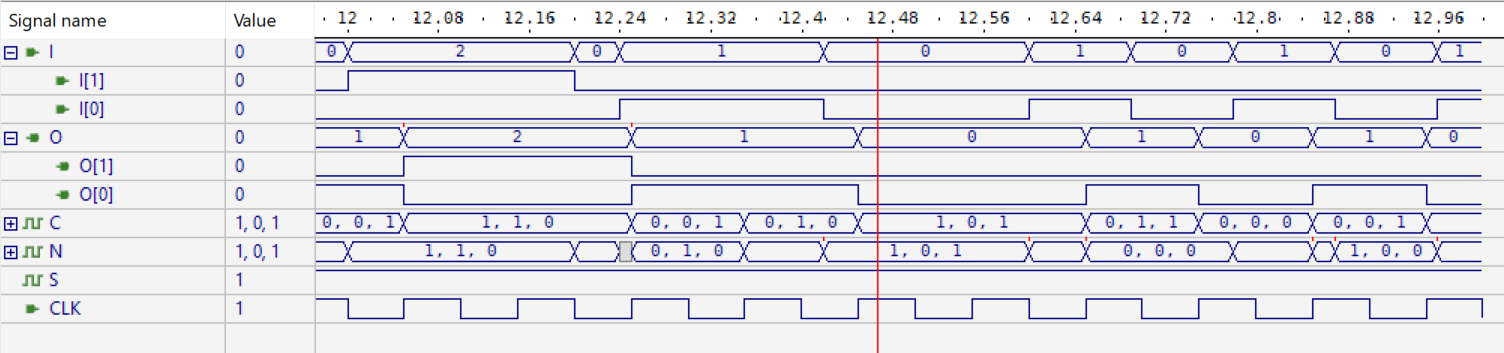
\includegraphics[width=\textwidth]{Figures/Test of FSM.png}
    \caption{Timing diagram of FSM simulated in Verilog}
    \label{fig:fsm_simulation}
\end{figure}

From the figure we see that the memory transitions to the expected states based on the inputs. The FSM begins in state ''Run-1'' and transitions to state ''Reset'' as the reset input $I_1$ is set high. The next state is ''Run-1'', then ''Run-2''. The Run-bit $I_0$ is then set low, resulting in a two-period pause in state ''Pause-2''. Further the FSM transitions to ''Run-3'', ''Pause'' and ''Run-1''.

This simulation was run and verified to follow the wanted behaviour as given by table~\ref{tab:truthtable}.

Present the results of your simulations in this section. Use tables and graphs or other figures to illustrate your results. Remember: The table caption goes above the table, the figure caption goes below the figure.

The results section must include:
\begin{itemize}
    \item Figures and/or tables that show the results of your simulation.
    \item Text that describe what we see in the simulation results (e.g. as expected we can see that XYZ which means the circuit functions as intended).
    \item NB! The result section is a \textit{what?}-section. \textit{What} where the results? \textit{What} do the figures/results mean? Any \textit{why}-questions you might want to write about and try to answer typically belong in the discussion section.
\end{itemize}